% Options for packages loaded elsewhere
\PassOptionsToPackage{unicode}{hyperref}
\PassOptionsToPackage{hyphens}{url}
\PassOptionsToPackage{dvipsnames,svgnames,x11names}{xcolor}
%
\documentclass[
  letterpaper,
  DIV=11,
  numbers=noendperiod]{scrartcl}

\usepackage{amsmath,amssymb}
\usepackage{iftex}
\ifPDFTeX
  \usepackage[T1]{fontenc}
  \usepackage[utf8]{inputenc}
  \usepackage{textcomp} % provide euro and other symbols
\else % if luatex or xetex
  \usepackage{unicode-math}
  \defaultfontfeatures{Scale=MatchLowercase}
  \defaultfontfeatures[\rmfamily]{Ligatures=TeX,Scale=1}
\fi
\usepackage{lmodern}
\ifPDFTeX\else  
    % xetex/luatex font selection
\fi
% Use upquote if available, for straight quotes in verbatim environments
\IfFileExists{upquote.sty}{\usepackage{upquote}}{}
\IfFileExists{microtype.sty}{% use microtype if available
  \usepackage[]{microtype}
  \UseMicrotypeSet[protrusion]{basicmath} % disable protrusion for tt fonts
}{}
\makeatletter
\@ifundefined{KOMAClassName}{% if non-KOMA class
  \IfFileExists{parskip.sty}{%
    \usepackage{parskip}
  }{% else
    \setlength{\parindent}{0pt}
    \setlength{\parskip}{6pt plus 2pt minus 1pt}}
}{% if KOMA class
  \KOMAoptions{parskip=half}}
\makeatother
\usepackage{xcolor}
\setlength{\emergencystretch}{3em} % prevent overfull lines
\setcounter{secnumdepth}{-\maxdimen} % remove section numbering
% Make \paragraph and \subparagraph free-standing
\makeatletter
\ifx\paragraph\undefined\else
  \let\oldparagraph\paragraph
  \renewcommand{\paragraph}{
    \@ifstar
      \xxxParagraphStar
      \xxxParagraphNoStar
  }
  \newcommand{\xxxParagraphStar}[1]{\oldparagraph*{#1}\mbox{}}
  \newcommand{\xxxParagraphNoStar}[1]{\oldparagraph{#1}\mbox{}}
\fi
\ifx\subparagraph\undefined\else
  \let\oldsubparagraph\subparagraph
  \renewcommand{\subparagraph}{
    \@ifstar
      \xxxSubParagraphStar
      \xxxSubParagraphNoStar
  }
  \newcommand{\xxxSubParagraphStar}[1]{\oldsubparagraph*{#1}\mbox{}}
  \newcommand{\xxxSubParagraphNoStar}[1]{\oldsubparagraph{#1}\mbox{}}
\fi
\makeatother

\usepackage{color}
\usepackage{fancyvrb}
\newcommand{\VerbBar}{|}
\newcommand{\VERB}{\Verb[commandchars=\\\{\}]}
\DefineVerbatimEnvironment{Highlighting}{Verbatim}{commandchars=\\\{\}}
% Add ',fontsize=\small' for more characters per line
\usepackage{framed}
\definecolor{shadecolor}{RGB}{241,243,245}
\newenvironment{Shaded}{\begin{snugshade}}{\end{snugshade}}
\newcommand{\AlertTok}[1]{\textcolor[rgb]{0.68,0.00,0.00}{#1}}
\newcommand{\AnnotationTok}[1]{\textcolor[rgb]{0.37,0.37,0.37}{#1}}
\newcommand{\AttributeTok}[1]{\textcolor[rgb]{0.40,0.45,0.13}{#1}}
\newcommand{\BaseNTok}[1]{\textcolor[rgb]{0.68,0.00,0.00}{#1}}
\newcommand{\BuiltInTok}[1]{\textcolor[rgb]{0.00,0.23,0.31}{#1}}
\newcommand{\CharTok}[1]{\textcolor[rgb]{0.13,0.47,0.30}{#1}}
\newcommand{\CommentTok}[1]{\textcolor[rgb]{0.37,0.37,0.37}{#1}}
\newcommand{\CommentVarTok}[1]{\textcolor[rgb]{0.37,0.37,0.37}{\textit{#1}}}
\newcommand{\ConstantTok}[1]{\textcolor[rgb]{0.56,0.35,0.01}{#1}}
\newcommand{\ControlFlowTok}[1]{\textcolor[rgb]{0.00,0.23,0.31}{\textbf{#1}}}
\newcommand{\DataTypeTok}[1]{\textcolor[rgb]{0.68,0.00,0.00}{#1}}
\newcommand{\DecValTok}[1]{\textcolor[rgb]{0.68,0.00,0.00}{#1}}
\newcommand{\DocumentationTok}[1]{\textcolor[rgb]{0.37,0.37,0.37}{\textit{#1}}}
\newcommand{\ErrorTok}[1]{\textcolor[rgb]{0.68,0.00,0.00}{#1}}
\newcommand{\ExtensionTok}[1]{\textcolor[rgb]{0.00,0.23,0.31}{#1}}
\newcommand{\FloatTok}[1]{\textcolor[rgb]{0.68,0.00,0.00}{#1}}
\newcommand{\FunctionTok}[1]{\textcolor[rgb]{0.28,0.35,0.67}{#1}}
\newcommand{\ImportTok}[1]{\textcolor[rgb]{0.00,0.46,0.62}{#1}}
\newcommand{\InformationTok}[1]{\textcolor[rgb]{0.37,0.37,0.37}{#1}}
\newcommand{\KeywordTok}[1]{\textcolor[rgb]{0.00,0.23,0.31}{\textbf{#1}}}
\newcommand{\NormalTok}[1]{\textcolor[rgb]{0.00,0.23,0.31}{#1}}
\newcommand{\OperatorTok}[1]{\textcolor[rgb]{0.37,0.37,0.37}{#1}}
\newcommand{\OtherTok}[1]{\textcolor[rgb]{0.00,0.23,0.31}{#1}}
\newcommand{\PreprocessorTok}[1]{\textcolor[rgb]{0.68,0.00,0.00}{#1}}
\newcommand{\RegionMarkerTok}[1]{\textcolor[rgb]{0.00,0.23,0.31}{#1}}
\newcommand{\SpecialCharTok}[1]{\textcolor[rgb]{0.37,0.37,0.37}{#1}}
\newcommand{\SpecialStringTok}[1]{\textcolor[rgb]{0.13,0.47,0.30}{#1}}
\newcommand{\StringTok}[1]{\textcolor[rgb]{0.13,0.47,0.30}{#1}}
\newcommand{\VariableTok}[1]{\textcolor[rgb]{0.07,0.07,0.07}{#1}}
\newcommand{\VerbatimStringTok}[1]{\textcolor[rgb]{0.13,0.47,0.30}{#1}}
\newcommand{\WarningTok}[1]{\textcolor[rgb]{0.37,0.37,0.37}{\textit{#1}}}

\providecommand{\tightlist}{%
  \setlength{\itemsep}{0pt}\setlength{\parskip}{0pt}}\usepackage{longtable,booktabs,array}
\usepackage{calc} % for calculating minipage widths
% Correct order of tables after \paragraph or \subparagraph
\usepackage{etoolbox}
\makeatletter
\patchcmd\longtable{\par}{\if@noskipsec\mbox{}\fi\par}{}{}
\makeatother
% Allow footnotes in longtable head/foot
\IfFileExists{footnotehyper.sty}{\usepackage{footnotehyper}}{\usepackage{footnote}}
\makesavenoteenv{longtable}
\usepackage{graphicx}
\makeatletter
\newsavebox\pandoc@box
\newcommand*\pandocbounded[1]{% scales image to fit in text height/width
  \sbox\pandoc@box{#1}%
  \Gscale@div\@tempa{\textheight}{\dimexpr\ht\pandoc@box+\dp\pandoc@box\relax}%
  \Gscale@div\@tempb{\linewidth}{\wd\pandoc@box}%
  \ifdim\@tempb\p@<\@tempa\p@\let\@tempa\@tempb\fi% select the smaller of both
  \ifdim\@tempa\p@<\p@\scalebox{\@tempa}{\usebox\pandoc@box}%
  \else\usebox{\pandoc@box}%
  \fi%
}
% Set default figure placement to htbp
\def\fps@figure{htbp}
\makeatother

\KOMAoption{captions}{tableheading}
\makeatletter
\@ifpackageloaded{caption}{}{\usepackage{caption}}
\AtBeginDocument{%
\ifdefined\contentsname
  \renewcommand*\contentsname{Table of contents}
\else
  \newcommand\contentsname{Table of contents}
\fi
\ifdefined\listfigurename
  \renewcommand*\listfigurename{List of Figures}
\else
  \newcommand\listfigurename{List of Figures}
\fi
\ifdefined\listtablename
  \renewcommand*\listtablename{List of Tables}
\else
  \newcommand\listtablename{List of Tables}
\fi
\ifdefined\figurename
  \renewcommand*\figurename{Figure}
\else
  \newcommand\figurename{Figure}
\fi
\ifdefined\tablename
  \renewcommand*\tablename{Table}
\else
  \newcommand\tablename{Table}
\fi
}
\@ifpackageloaded{float}{}{\usepackage{float}}
\floatstyle{ruled}
\@ifundefined{c@chapter}{\newfloat{codelisting}{h}{lop}}{\newfloat{codelisting}{h}{lop}[chapter]}
\floatname{codelisting}{Listing}
\newcommand*\listoflistings{\listof{codelisting}{List of Listings}}
\makeatother
\makeatletter
\makeatother
\makeatletter
\@ifpackageloaded{caption}{}{\usepackage{caption}}
\@ifpackageloaded{subcaption}{}{\usepackage{subcaption}}
\makeatother

\usepackage{bookmark}

\IfFileExists{xurl.sty}{\usepackage{xurl}}{} % add URL line breaks if available
\urlstyle{same} % disable monospaced font for URLs
\hypersetup{
  pdftitle={Lab 5 Solutions: Continuous Random Variables \& Confidence Intervals},
  pdfauthor={Complete Solutions Guide},
  colorlinks=true,
  linkcolor={blue},
  filecolor={Maroon},
  citecolor={Blue},
  urlcolor={Blue},
  pdfcreator={LaTeX via pandoc}}


\title{Lab 5 Solutions: Continuous Random Variables \& Confidence
Intervals}
\usepackage{etoolbox}
\makeatletter
\providecommand{\subtitle}[1]{% add subtitle to \maketitle
  \apptocmd{\@title}{\par {\large #1 \par}}{}{}
}
\makeatother
\subtitle{PSTAT 5A - Summer Session A 2025}
\author{Complete Solutions Guide}
\date{2025-07-22}

\begin{document}
\maketitle

\renewcommand*\contentsname{Table of contents}
{
\hypersetup{linkcolor=}
\setcounter{tocdepth}{3}
\tableofcontents
}

\section{Getting Started - Setup
Code}\label{getting-started---setup-code}

\begin{Shaded}
\begin{Highlighting}[]
\CommentTok{\# Install any missing packages (will skip those already installed)}
\CommentTok{\#!\%pip install {-}{-}quiet numpy matplotlib scipy pandas statsmodels}

\CommentTok{\# Load our tools (libraries)}
\ImportTok{import}\NormalTok{ numpy }\ImportTok{as}\NormalTok{ np }\CommentTok{\# numerical computing (arrays, random numbers, etc.)}
\ImportTok{import}\NormalTok{ matplotlib.pyplot }\ImportTok{as}\NormalTok{ plt }\CommentTok{\# plotting library for static 2D graphs and visualizations}
\ImportTok{from}\NormalTok{ scipy }\ImportTok{import}\NormalTok{ stats }\CommentTok{\#  statistical functions (distributions, tests, etc.)}
\ImportTok{import}\NormalTok{ pandas }\ImportTok{as}\NormalTok{ pd }\CommentTok{\# data structures (DataFrame) and data analysis tools}
\ImportTok{import}\NormalTok{ statsmodels  }\CommentTok{\# statistical modeling (regression, time series, ANOVA, etc.)}

\CommentTok{\# Make our graphs look nice}
\CommentTok{\#!\%matplotlib inline     \# embed Matplotlib plots directly in the notebook}
\NormalTok{plt.style.use(}\StringTok{\textquotesingle{}seaborn{-}v0\_8{-}whitegrid\textquotesingle{}}\NormalTok{)  }\CommentTok{\# Apply a clean whitegrid style from Seaborn}

\CommentTok{\# Set random seed for reproducible results}
\NormalTok{np.random.seed(}\DecValTok{42}\NormalTok{)    }\CommentTok{\# fix the random seed so results can be reproduced exactly}

\BuiltInTok{print}\NormalTok{(}\StringTok{"✅ All tools loaded successfully!"}\NormalTok{) }
\end{Highlighting}
\end{Shaded}

\begin{verbatim}
✅ All tools loaded successfully!
\end{verbatim}

\section{Task 1 Solution: Your First Normal
Distribution}\label{task-1-solution-your-first-normal-distribution}

Human heights follow a normal distribution with mean = 68 inches and
standard deviation = 4 inches.

\begin{Shaded}
\begin{Highlighting}[]
\CommentTok{\# Heights distribution {-} SOLUTION}
\NormalTok{mean\_height }\OperatorTok{=} \DecValTok{68}  \CommentTok{\# SOLUTION: 68}
\NormalTok{std\_height }\OperatorTok{=} \DecValTok{4}    \CommentTok{\# SOLUTION: 4}

\NormalTok{heights }\OperatorTok{=}\NormalTok{ stats.norm(loc}\OperatorTok{=}\NormalTok{mean\_height, scale}\OperatorTok{=}\NormalTok{std\_height)}

\BuiltInTok{print}\NormalTok{(}\SpecialStringTok{f"Mean height: }\SpecialCharTok{\{}\NormalTok{heights}\SpecialCharTok{.}\NormalTok{mean()}\SpecialCharTok{\}}\SpecialStringTok{ inches"}\NormalTok{)}
\BuiltInTok{print}\NormalTok{(}\SpecialStringTok{f"Standard deviation: }\SpecialCharTok{\{}\NormalTok{heights}\SpecialCharTok{.}\NormalTok{std()}\SpecialCharTok{\}}\SpecialStringTok{ inches"}\NormalTok{)}
\end{Highlighting}
\end{Shaded}

\begin{verbatim}
Mean height: 68.0 inches
Standard deviation: 4.0 inches
\end{verbatim}

\begin{Shaded}
\begin{Highlighting}[]
\CommentTok{\# Calculate probabilities {-} SOLUTION}

\CommentTok{\# a) What\textquotesingle{}s the probability someone is taller than 72 inches (6 feet)?}
\NormalTok{prob\_tall }\OperatorTok{=} \DecValTok{1} \OperatorTok{{-}}\NormalTok{ heights.cdf(}\DecValTok{72}\NormalTok{)  }\CommentTok{\# SOLUTION: 72}
\BuiltInTok{print}\NormalTok{(}\SpecialStringTok{f"P(height \textgreater{} 72 inches) = }\SpecialCharTok{\{}\NormalTok{prob\_tall}\SpecialCharTok{:.4f\}}\SpecialStringTok{"}\NormalTok{)}

\CommentTok{\# b) What\textquotesingle{}s the probability someone is between 64 and 72 inches?}
\NormalTok{prob\_between }\OperatorTok{=}\NormalTok{ heights.cdf(}\DecValTok{72}\NormalTok{) }\OperatorTok{{-}}\NormalTok{ heights.cdf(}\DecValTok{64}\NormalTok{)  }\CommentTok{\# SOLUTION: 72, 64}
\BuiltInTok{print}\NormalTok{(}\SpecialStringTok{f"P(64 \textless{} height \textless{} 72) = }\SpecialCharTok{\{}\NormalTok{prob\_between}\SpecialCharTok{:.4f\}}\SpecialStringTok{"}\NormalTok{)}

\CommentTok{\# c) What height is at the 90th percentile? (90\% of people are shorter)}
\NormalTok{height\_90th }\OperatorTok{=}\NormalTok{ heights.ppf(}\FloatTok{0.90}\NormalTok{)  }\CommentTok{\# SOLUTION: 0.90}
\BuiltInTok{print}\NormalTok{(}\SpecialStringTok{f"90th percentile height: }\SpecialCharTok{\{}\NormalTok{height\_90th}\SpecialCharTok{:.2f\}}\SpecialStringTok{ inches"}\NormalTok{)}
\end{Highlighting}
\end{Shaded}

\begin{verbatim}
P(height > 72 inches) = 0.1587
P(64 < height < 72) = 0.6827
90th percentile height: 73.13 inches
\end{verbatim}

\begin{Shaded}
\begin{Highlighting}[]
\CommentTok{\# Visualization {-} SOLUTION}
\NormalTok{x }\OperatorTok{=}\NormalTok{ np.linspace(}\DecValTok{50}\NormalTok{, }\DecValTok{86}\NormalTok{, }\DecValTok{1000}\NormalTok{)}
\NormalTok{y }\OperatorTok{=}\NormalTok{ heights.pdf(x)}

\NormalTok{plt.figure(figsize}\OperatorTok{=}\NormalTok{(}\DecValTok{10}\NormalTok{, }\DecValTok{6}\NormalTok{))}
\NormalTok{plt.plot(x, y, }\StringTok{\textquotesingle{}b{-}\textquotesingle{}}\NormalTok{, linewidth}\OperatorTok{=}\DecValTok{2}\NormalTok{)}
\NormalTok{plt.fill\_between(x, y, alpha}\OperatorTok{=}\FloatTok{0.3}\NormalTok{, color}\OperatorTok{=}\StringTok{\textquotesingle{}lightgreen\textquotesingle{}}\NormalTok{)}
\NormalTok{plt.title(}\StringTok{\textquotesingle{}Human Heights Distribution\textquotesingle{}}\NormalTok{)}
\NormalTok{plt.xlabel(}\StringTok{\textquotesingle{}Height (inches)\textquotesingle{}}\NormalTok{)}
\NormalTok{plt.ylabel(}\StringTok{\textquotesingle{}Density\textquotesingle{}}\NormalTok{)}
\NormalTok{plt.axvline(mean\_height, color}\OperatorTok{=}\StringTok{\textquotesingle{}red\textquotesingle{}}\NormalTok{, linestyle}\OperatorTok{=}\StringTok{\textquotesingle{}{-}{-}\textquotesingle{}}\NormalTok{, linewidth}\OperatorTok{=}\DecValTok{2}\NormalTok{, }
\NormalTok{           label}\OperatorTok{=}\SpecialStringTok{f\textquotesingle{}Mean = }\SpecialCharTok{\{}\NormalTok{mean\_height}\SpecialCharTok{\}}\SpecialStringTok{ inches\textquotesingle{}}\NormalTok{)}
\NormalTok{plt.legend()}
\NormalTok{plt.grid(}\VariableTok{True}\NormalTok{, alpha}\OperatorTok{=}\FloatTok{0.3}\NormalTok{)}
\NormalTok{plt.show()}
\end{Highlighting}
\end{Shaded}

\pandocbounded{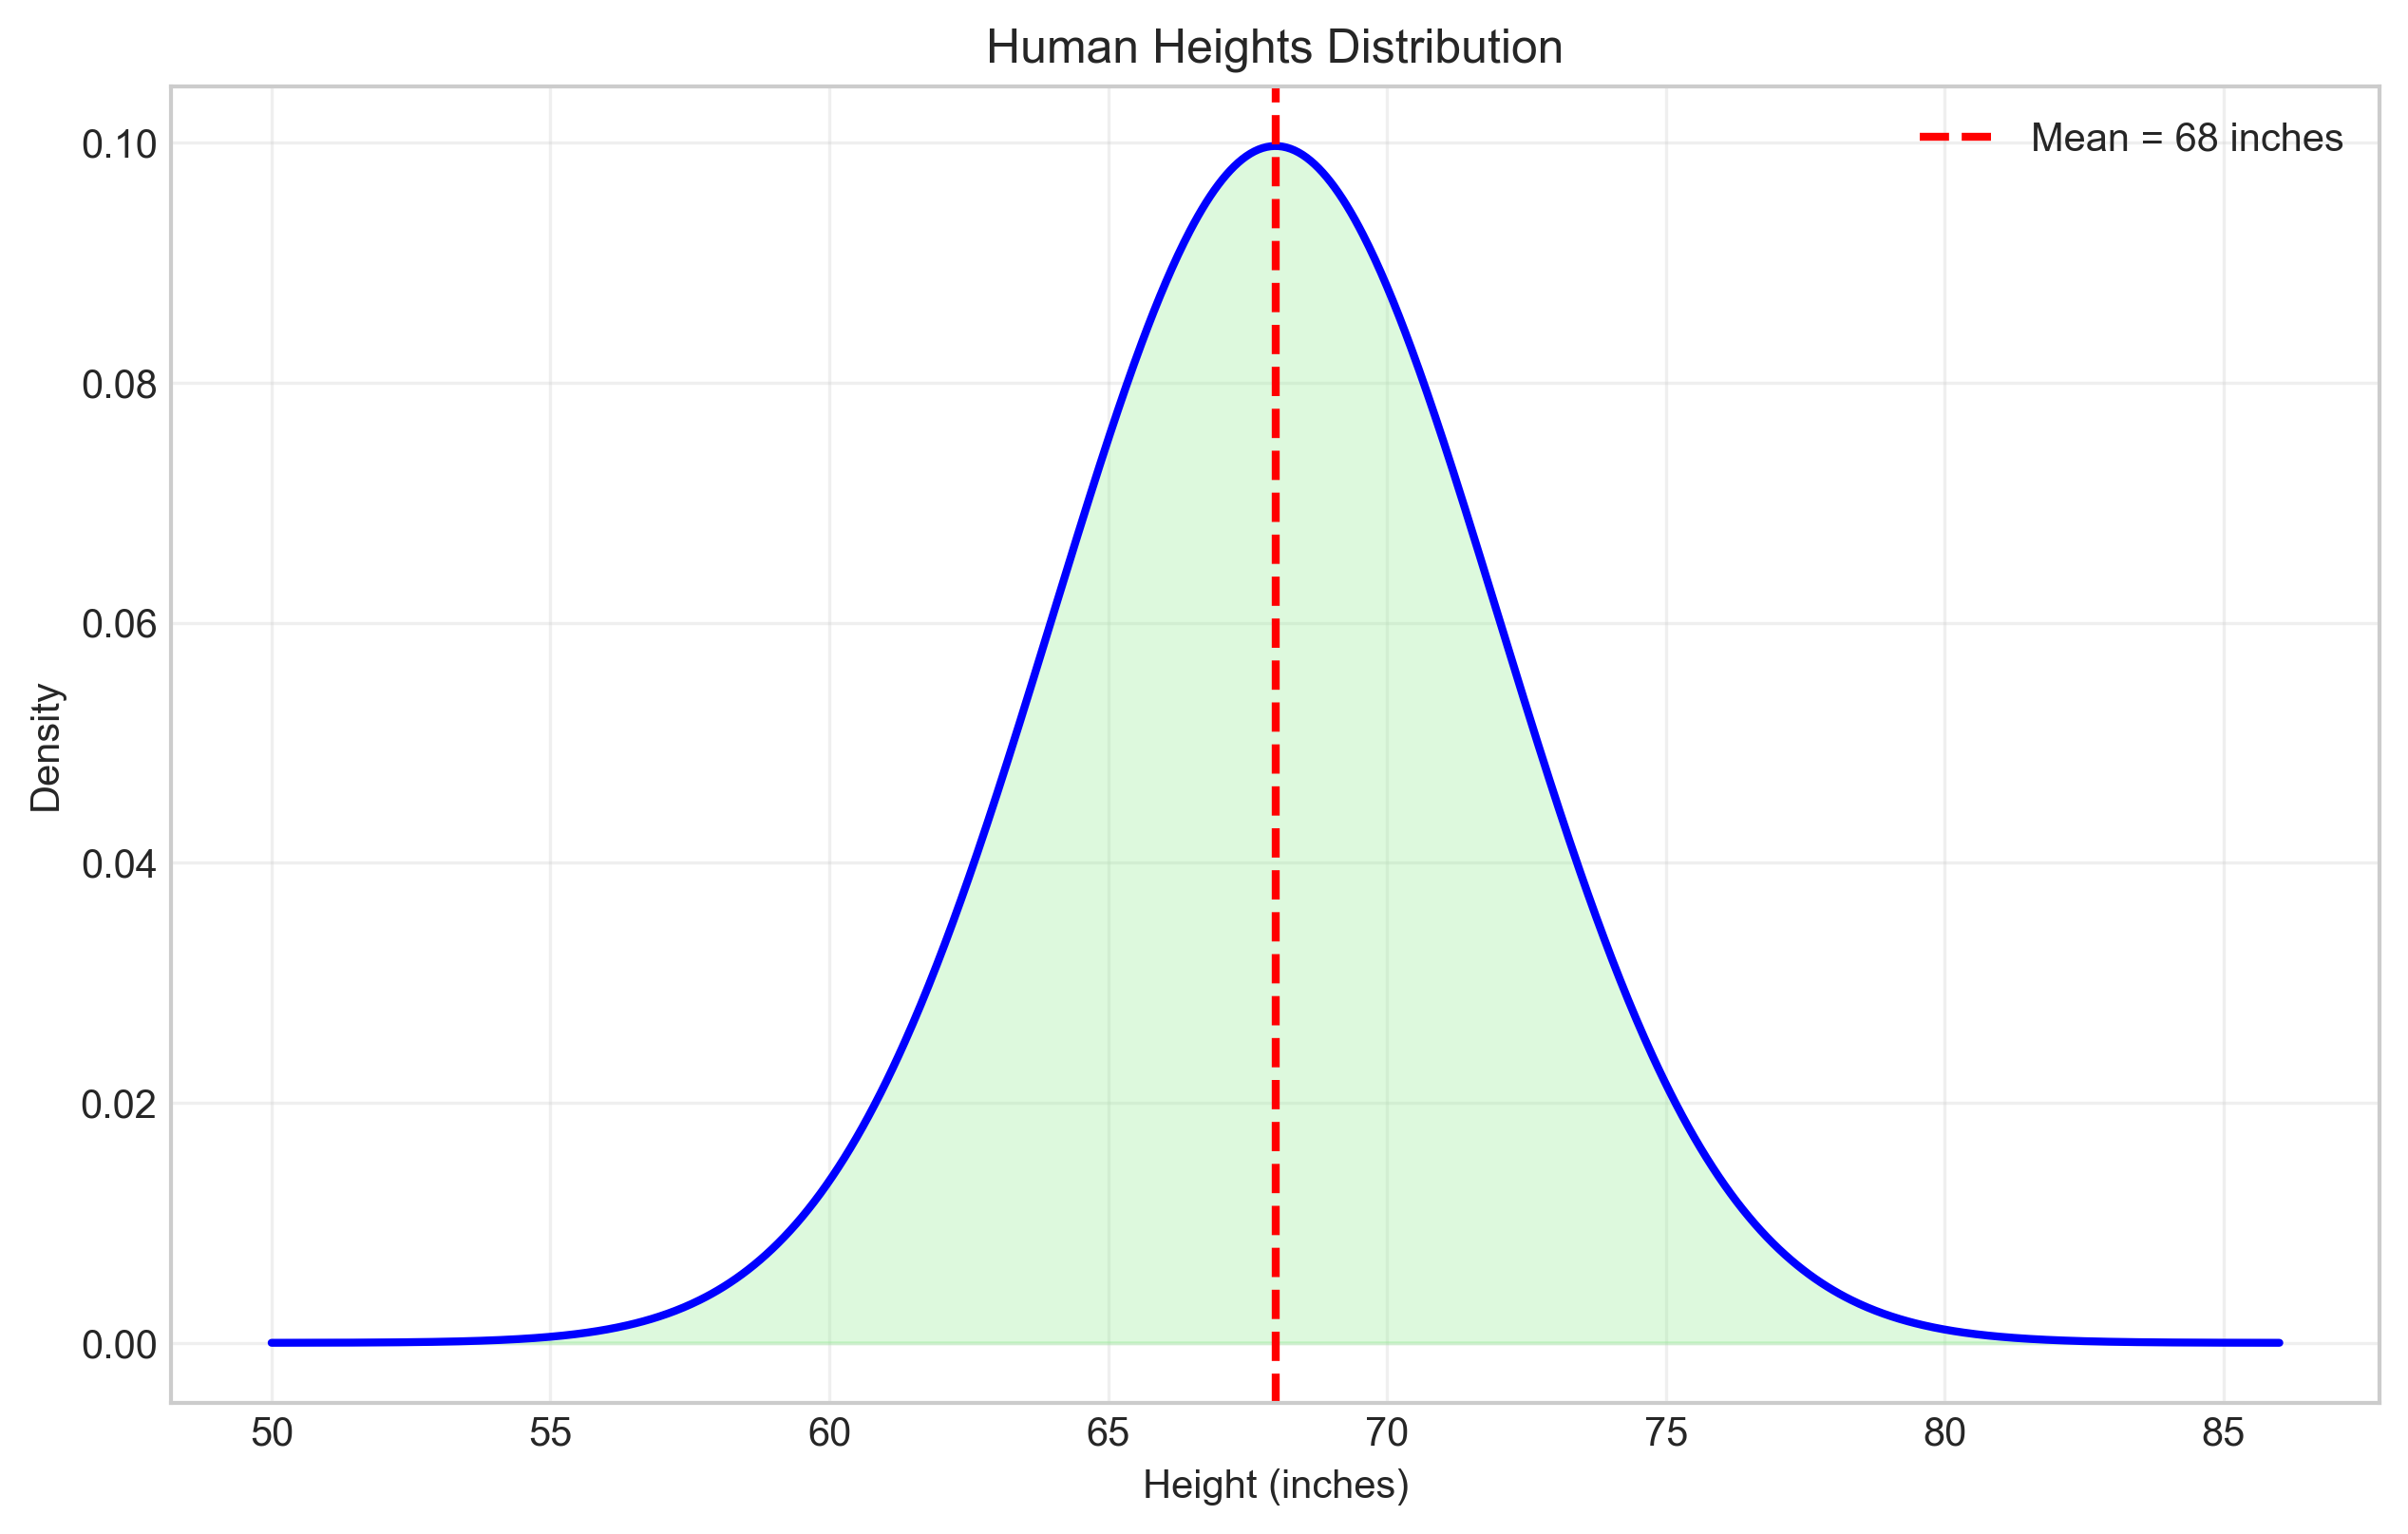
\includegraphics[keepaspectratio]{lab5_sln_files/figure-pdf/cell-5-output-1.png}}

\section{Task 2 Solution: Bus Waiting
Times}\label{task-2-solution-bus-waiting-times}

The time between buses follows an exponential distribution with an
average of 15 minutes between buses.

\begin{Shaded}
\begin{Highlighting}[]
\CommentTok{\# Bus waiting times {-} SOLUTION}
\NormalTok{average\_wait }\OperatorTok{=} \DecValTok{15}  \CommentTok{\# SOLUTION: 15 minutes}
\NormalTok{rate }\OperatorTok{=} \DecValTok{1} \OperatorTok{/}\NormalTok{ average\_wait}
\NormalTok{bus\_times }\OperatorTok{=}\NormalTok{ stats.expon(scale}\OperatorTok{=}\NormalTok{average\_wait)  }\CommentTok{\# SOLUTION: average\_wait}

\CommentTok{\# Questions:}
\CommentTok{\# a) What\textquotesingle{}s the probability you wait less than 10 minutes?}
\NormalTok{prob\_short }\OperatorTok{=}\NormalTok{ bus\_times.cdf(}\DecValTok{10}\NormalTok{)  }\CommentTok{\# SOLUTION: 10}
\BuiltInTok{print}\NormalTok{(}\SpecialStringTok{f"P(wait \textless{} 10 min) = }\SpecialCharTok{\{}\NormalTok{prob\_short}\SpecialCharTok{:.4f\}}\SpecialStringTok{"}\NormalTok{)}

\CommentTok{\# b) What\textquotesingle{}s the probability you wait more than 30 minutes?}
\NormalTok{prob\_long }\OperatorTok{=} \DecValTok{1} \OperatorTok{{-}}\NormalTok{ bus\_times.cdf(}\DecValTok{30}\NormalTok{)  }\CommentTok{\# SOLUTION: 30}
\BuiltInTok{print}\NormalTok{(}\SpecialStringTok{f"P(wait \textgreater{} 30 min) = }\SpecialCharTok{\{}\NormalTok{prob\_long}\SpecialCharTok{:.4f\}}\SpecialStringTok{"}\NormalTok{)}

\CommentTok{\# c) What\textquotesingle{}s the median waiting time? (50th percentile)}
\NormalTok{median\_wait }\OperatorTok{=}\NormalTok{ bus\_times.ppf(}\FloatTok{0.5}\NormalTok{)  }\CommentTok{\# SOLUTION: 0.5}
\BuiltInTok{print}\NormalTok{(}\SpecialStringTok{f"Median wait time: }\SpecialCharTok{\{}\NormalTok{median\_wait}\SpecialCharTok{:.2f\}}\SpecialStringTok{ minutes"}\NormalTok{)}
\end{Highlighting}
\end{Shaded}

\begin{verbatim}
P(wait < 10 min) = 0.4866
P(wait > 30 min) = 0.1353
Median wait time: 10.40 minutes
\end{verbatim}

\section{Task 3 Solution: Explore the
CLT}\label{task-3-solution-explore-the-clt}

Let's verify the Central Limit Theorem with a uniform distribution!

\begin{Shaded}
\begin{Highlighting}[]
\CommentTok{\# Population: Uniform distribution from 0 to 100 {-} SOLUTION}
\NormalTok{population }\OperatorTok{=}\NormalTok{ stats.uniform(loc}\OperatorTok{=}\DecValTok{0}\NormalTok{, scale}\OperatorTok{=}\DecValTok{100}\NormalTok{)}

\BuiltInTok{print}\NormalTok{(}\StringTok{"Population (Uniform 0 to 100):"}\NormalTok{)}
\BuiltInTok{print}\NormalTok{(}\SpecialStringTok{f"Population mean: }\SpecialCharTok{\{}\NormalTok{population}\SpecialCharTok{.}\NormalTok{mean()}\SpecialCharTok{\}}\SpecialStringTok{"}\NormalTok{)}
\BuiltInTok{print}\NormalTok{(}\SpecialStringTok{f"Population std: }\SpecialCharTok{\{}\NormalTok{population}\SpecialCharTok{.}\NormalTok{std()}\SpecialCharTok{:.2f\}}\SpecialStringTok{"}\NormalTok{)}

\CommentTok{\# Take 500 samples of size 25 each {-} SOLUTION}
\NormalTok{sample\_size }\OperatorTok{=} \DecValTok{25}   \CommentTok{\# SOLUTION: 25}
\NormalTok{n\_samples }\OperatorTok{=} \DecValTok{500}    \CommentTok{\# SOLUTION: 500}

\NormalTok{sample\_means }\OperatorTok{=}\NormalTok{ []}
\ControlFlowTok{for}\NormalTok{ i }\KeywordTok{in} \BuiltInTok{range}\NormalTok{(n\_samples):}
\NormalTok{    sample }\OperatorTok{=}\NormalTok{ population.rvs(sample\_size)  }\CommentTok{\# SOLUTION: sample\_size}
\NormalTok{    sample\_means.append(np.mean(sample))}

\CommentTok{\# Check the CLT prediction}
\NormalTok{predicted\_mean }\OperatorTok{=}\NormalTok{ population.mean()}
\NormalTok{predicted\_std }\OperatorTok{=}\NormalTok{ population.std() }\OperatorTok{/}\NormalTok{ np.sqrt(sample\_size)}

\BuiltInTok{print}\NormalTok{(}\SpecialStringTok{f"}\CharTok{\textbackslash{}n}\SpecialStringTok{CLT Predictions:"}\NormalTok{)}
\BuiltInTok{print}\NormalTok{(}\SpecialStringTok{f"Sample means should have mean ≈ }\SpecialCharTok{\{}\NormalTok{predicted\_mean}\SpecialCharTok{:.2f\}}\SpecialStringTok{"}\NormalTok{)}
\BuiltInTok{print}\NormalTok{(}\SpecialStringTok{f"Sample means should have std ≈ }\SpecialCharTok{\{}\NormalTok{predicted\_std}\SpecialCharTok{:.2f\}}\SpecialStringTok{"}\NormalTok{)}

\BuiltInTok{print}\NormalTok{(}\SpecialStringTok{f"}\CharTok{\textbackslash{}n}\SpecialStringTok{Actual Results:"}\NormalTok{)}
\BuiltInTok{print}\NormalTok{(}\SpecialStringTok{f"Sample means actually have mean = }\SpecialCharTok{\{}\NormalTok{np}\SpecialCharTok{.}\NormalTok{mean(sample\_means)}\SpecialCharTok{:.2f\}}\SpecialStringTok{"}\NormalTok{)}
\BuiltInTok{print}\NormalTok{(}\SpecialStringTok{f"Sample means actually have std = }\SpecialCharTok{\{}\NormalTok{np}\SpecialCharTok{.}\NormalTok{std(sample\_means)}\SpecialCharTok{:.2f\}}\SpecialStringTok{"}\NormalTok{)}

\CommentTok{\# Make a histogram}
\NormalTok{plt.figure(figsize}\OperatorTok{=}\NormalTok{(}\DecValTok{10}\NormalTok{, }\DecValTok{6}\NormalTok{))}
\NormalTok{plt.hist(sample\_means, bins}\OperatorTok{=}\DecValTok{30}\NormalTok{, density}\OperatorTok{=}\VariableTok{True}\NormalTok{, alpha}\OperatorTok{=}\FloatTok{0.7}\NormalTok{, color}\OperatorTok{=}\StringTok{\textquotesingle{}purple\textquotesingle{}}\NormalTok{, edgecolor}\OperatorTok{=}\StringTok{\textquotesingle{}black\textquotesingle{}}\NormalTok{)}
\NormalTok{plt.title(}\StringTok{\textquotesingle{}Distribution of Sample Means from Uniform Population\textquotesingle{}}\NormalTok{)}
\NormalTok{plt.xlabel(}\StringTok{\textquotesingle{}Sample Mean\textquotesingle{}}\NormalTok{)}
\NormalTok{plt.ylabel(}\StringTok{\textquotesingle{}Density\textquotesingle{}}\NormalTok{)}
\NormalTok{plt.axvline(np.mean(sample\_means), color}\OperatorTok{=}\StringTok{\textquotesingle{}red\textquotesingle{}}\NormalTok{, linestyle}\OperatorTok{=}\StringTok{\textquotesingle{}{-}{-}\textquotesingle{}}\NormalTok{, linewidth}\OperatorTok{=}\DecValTok{2}\NormalTok{, }
\NormalTok{           label}\OperatorTok{=}\SpecialStringTok{f\textquotesingle{}Actual mean = }\SpecialCharTok{\{}\NormalTok{np}\SpecialCharTok{.}\NormalTok{mean(sample\_means)}\SpecialCharTok{:.2f\}}\SpecialStringTok{\textquotesingle{}}\NormalTok{)}
\NormalTok{plt.legend()}
\NormalTok{plt.grid(}\VariableTok{True}\NormalTok{, alpha}\OperatorTok{=}\FloatTok{0.3}\NormalTok{)}
\NormalTok{plt.show()}
\end{Highlighting}
\end{Shaded}

\begin{verbatim}
Population (Uniform 0 to 100):
Population mean: 50.0
Population std: 28.87

CLT Predictions:
Sample means should have mean ≈ 50.00
Sample means should have std ≈ 5.77

Actual Results:
Sample means actually have mean = 49.63
Sample means actually have std = 5.29
\end{verbatim}

\pandocbounded{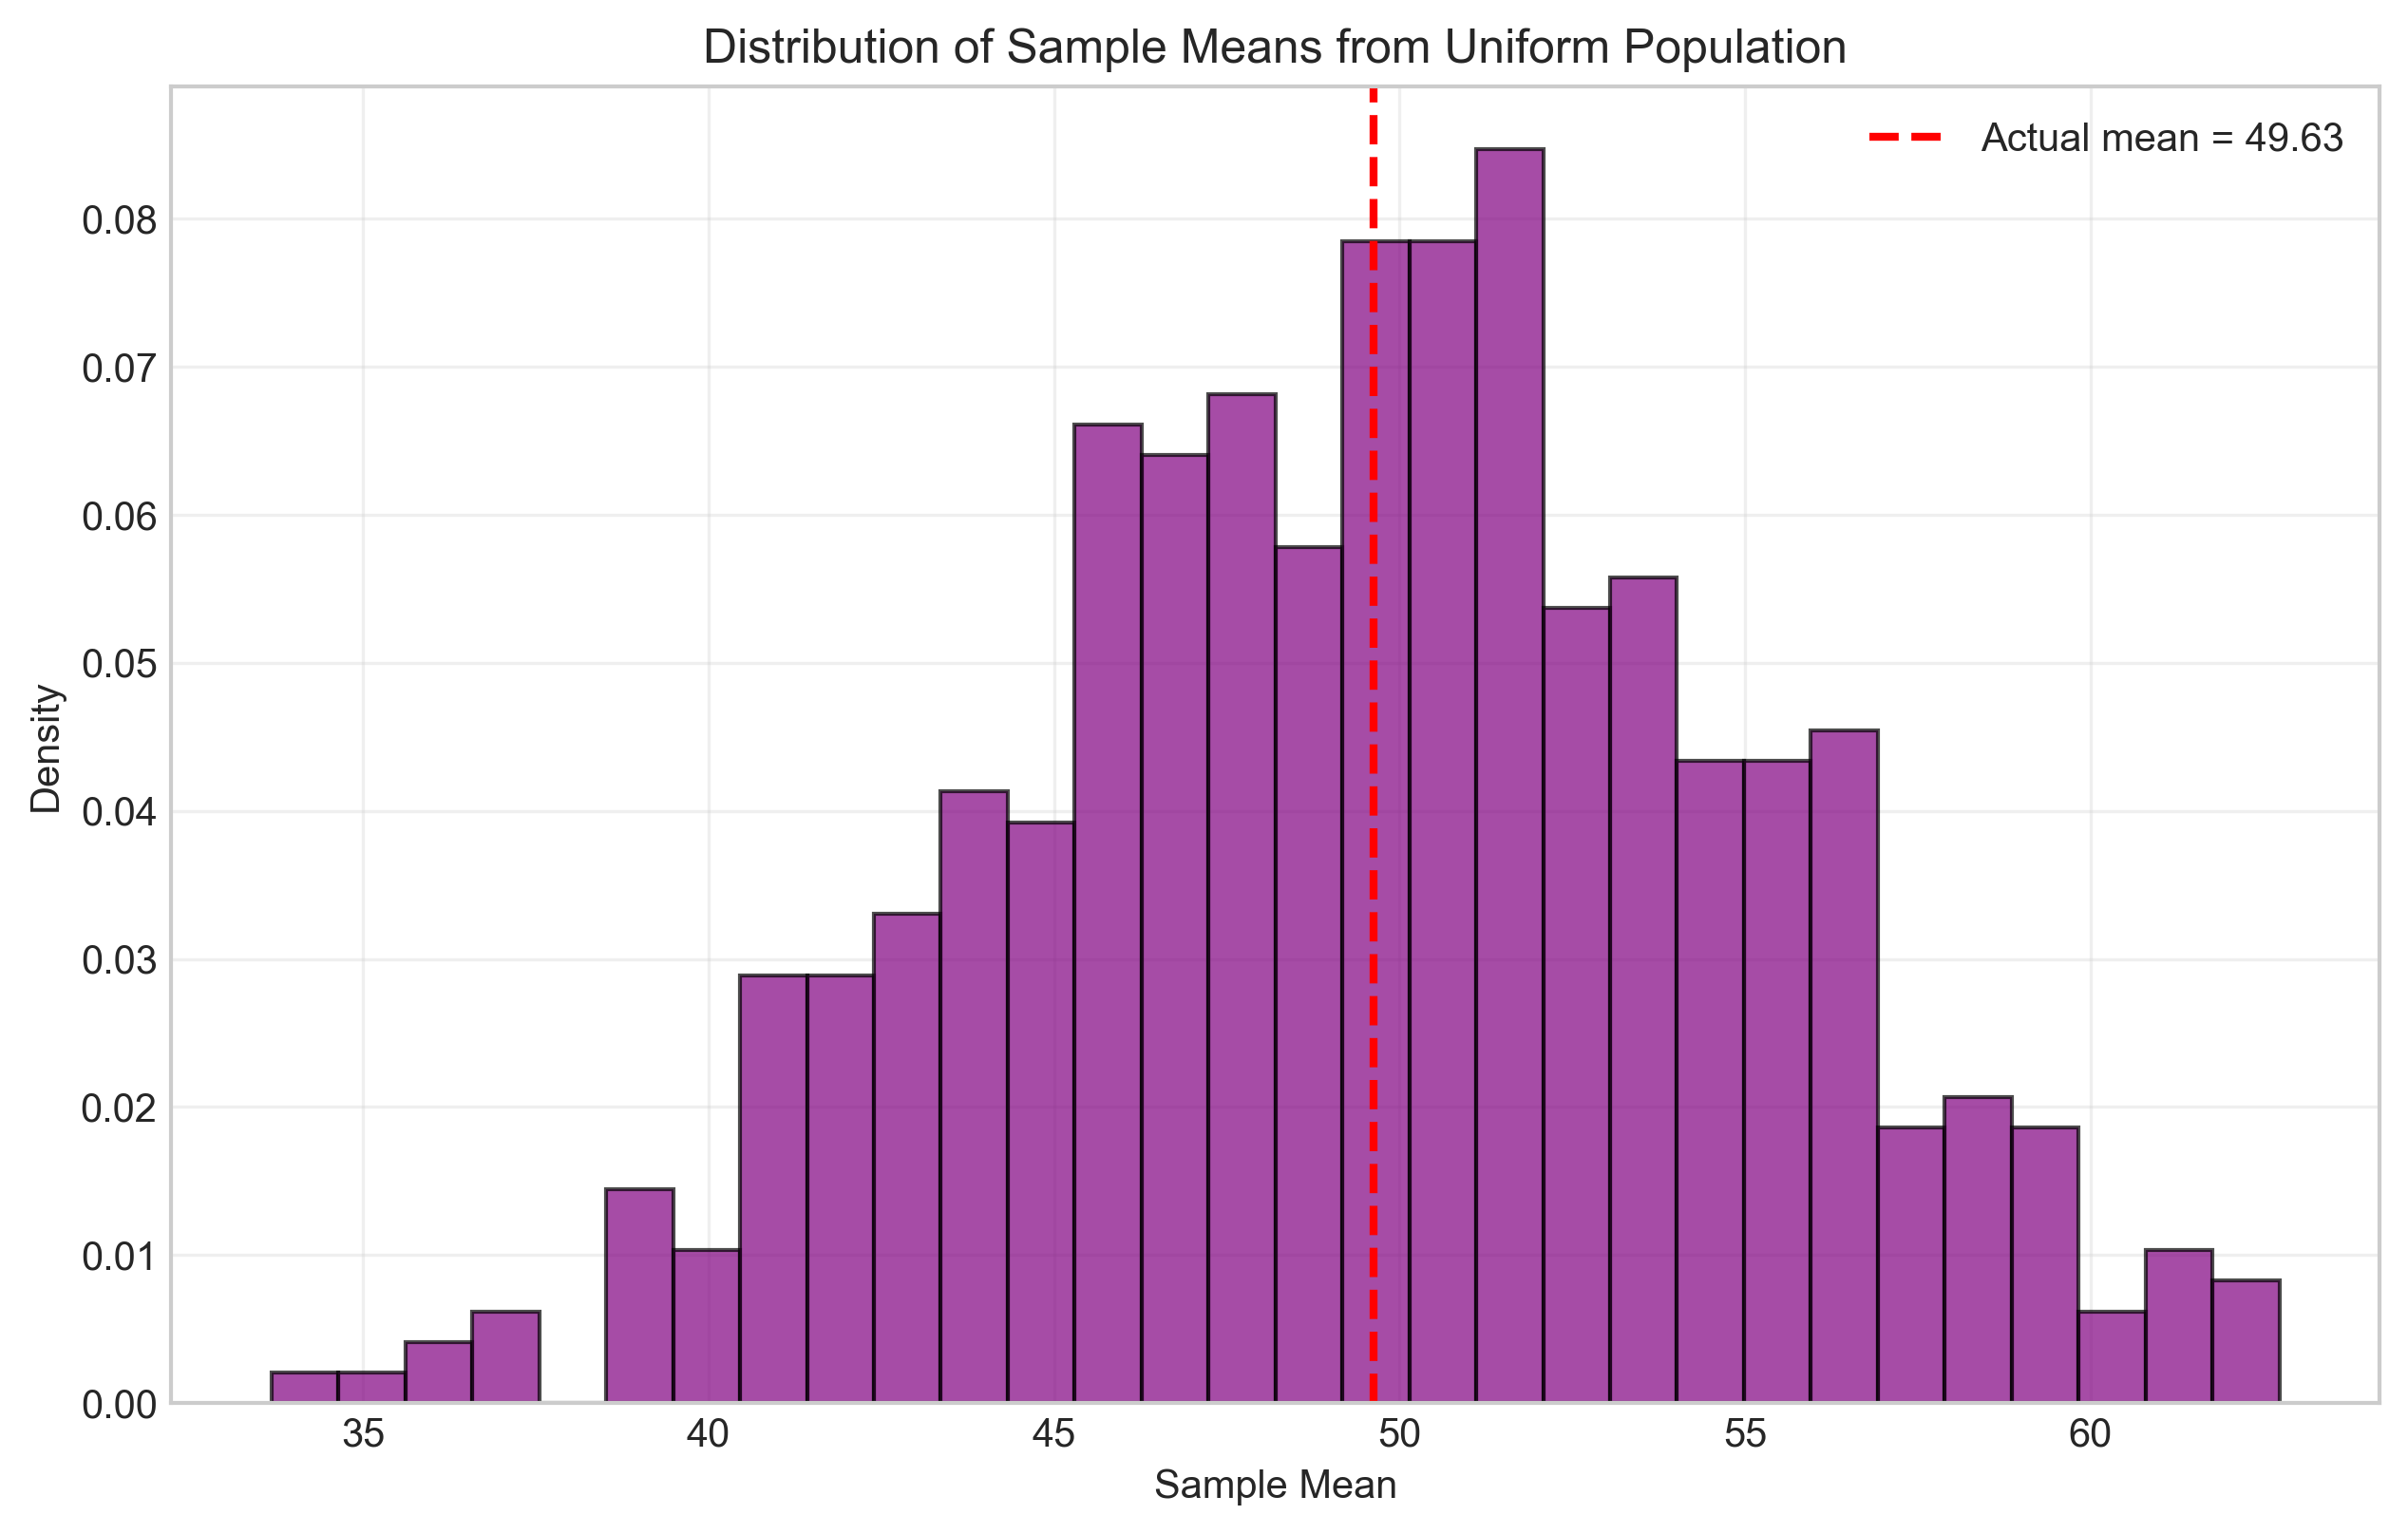
\includegraphics[keepaspectratio]{lab5_sln_files/figure-pdf/cell-7-output-2.png}}

\section{Task 4 Solution: Your Own Confidence
Interval}\label{task-4-solution-your-own-confidence-interval}

Creating a 90\% confidence interval for homework time data.

\begin{Shaded}
\begin{Highlighting}[]
\CommentTok{\# Homework time data (in hours per week) {-} SOLUTION}
\NormalTok{np.random.seed(}\DecValTok{456}\NormalTok{)}
\NormalTok{homework\_data }\OperatorTok{=}\NormalTok{ np.random.normal(}\DecValTok{15}\NormalTok{, }\DecValTok{5}\NormalTok{, }\DecValTok{40}\NormalTok{)  }\CommentTok{\# 40 students, roughly normal}

\BuiltInTok{print}\NormalTok{(}\StringTok{"Homework Survey Results:"}\NormalTok{)}
\BuiltInTok{print}\NormalTok{(}\SpecialStringTok{f"Sample size: }\SpecialCharTok{\{}\BuiltInTok{len}\NormalTok{(homework\_data)}\SpecialCharTok{\}}\SpecialStringTok{"}\NormalTok{)}
\BuiltInTok{print}\NormalTok{(}\SpecialStringTok{f"Sample mean: }\SpecialCharTok{\{}\NormalTok{np}\SpecialCharTok{.}\NormalTok{mean(homework\_data)}\SpecialCharTok{:.2f\}}\SpecialStringTok{ hours/week"}\NormalTok{)}
\BuiltInTok{print}\NormalTok{(}\SpecialStringTok{f"Sample std dev: }\SpecialCharTok{\{}\NormalTok{np}\SpecialCharTok{.}\NormalTok{std(homework\_data, ddof}\OperatorTok{=}\DecValTok{1}\NormalTok{)}\SpecialCharTok{:.2f\}}\SpecialStringTok{ hours/week"}\NormalTok{)}

\CommentTok{\# Create a 90\% confidence interval {-} SOLUTION}
\CommentTok{\# Step 1: Calculate the needed values}
\NormalTok{sample\_mean }\OperatorTok{=}\NormalTok{ np.mean(homework\_data)}
\NormalTok{sample\_std }\OperatorTok{=}\NormalTok{ np.std(homework\_data, ddof}\OperatorTok{=}\DecValTok{1}\NormalTok{)}
\NormalTok{n }\OperatorTok{=} \BuiltInTok{len}\NormalTok{(homework\_data)}

\CommentTok{\# Step 2: Find the critical value for 90\% confidence}
\NormalTok{confidence }\OperatorTok{=} \FloatTok{0.90}
\NormalTok{alpha }\OperatorTok{=} \DecValTok{1} \OperatorTok{{-}}\NormalTok{ confidence}
\NormalTok{z\_star }\OperatorTok{=}\NormalTok{ stats.norm.ppf(}\DecValTok{1} \OperatorTok{{-}}\NormalTok{ alpha}\OperatorTok{/}\DecValTok{2}\NormalTok{)}
\BuiltInTok{print}\NormalTok{(}\SpecialStringTok{f"Critical value for 90\% confidence: }\SpecialCharTok{\{}\NormalTok{z\_star}\SpecialCharTok{:.3f\}}\SpecialStringTok{"}\NormalTok{)}

\CommentTok{\# Step 3: Calculate standard error and margin of error}
\NormalTok{standard\_error }\OperatorTok{=}\NormalTok{ sample\_std }\OperatorTok{/}\NormalTok{ np.sqrt(n)}
\NormalTok{margin\_of\_error }\OperatorTok{=}\NormalTok{ z\_star }\OperatorTok{*}\NormalTok{ standard\_error}

\BuiltInTok{print}\NormalTok{(}\SpecialStringTok{f"Standard error: }\SpecialCharTok{\{}\NormalTok{standard\_error}\SpecialCharTok{:.3f\}}\SpecialStringTok{"}\NormalTok{)}
\BuiltInTok{print}\NormalTok{(}\SpecialStringTok{f"Margin of error: }\SpecialCharTok{\{}\NormalTok{margin\_of\_error}\SpecialCharTok{:.3f\}}\SpecialStringTok{"}\NormalTok{)}

\CommentTok{\# Step 4: Build the confidence interval}
\NormalTok{ci\_lower }\OperatorTok{=}\NormalTok{ sample\_mean }\OperatorTok{{-}}\NormalTok{ margin\_of\_error}
\NormalTok{ci\_upper }\OperatorTok{=}\NormalTok{ sample\_mean }\OperatorTok{+}\NormalTok{ margin\_of\_error}

\BuiltInTok{print}\NormalTok{(}\SpecialStringTok{f"}\CharTok{\textbackslash{}n}\SpecialStringTok{90\% Confidence Interval for average homework time:"}\NormalTok{)}
\BuiltInTok{print}\NormalTok{(}\SpecialStringTok{f"[}\SpecialCharTok{\{}\NormalTok{ci\_lower}\SpecialCharTok{:.2f\}}\SpecialStringTok{, }\SpecialCharTok{\{}\NormalTok{ci\_upper}\SpecialCharTok{:.2f\}}\SpecialStringTok{] hours per week"}\NormalTok{)}

\CommentTok{\# Step 5: Interpret your result}
\BuiltInTok{print}\NormalTok{(}\SpecialStringTok{f"}\CharTok{\textbackslash{}n}\SpecialStringTok{Interpretation:"}\NormalTok{)}
\BuiltInTok{print}\NormalTok{(}\SpecialStringTok{f"We are 90\% confident that the true average homework time"}\NormalTok{)}
\BuiltInTok{print}\NormalTok{(}\SpecialStringTok{f"for all students is between }\SpecialCharTok{\{}\NormalTok{ci\_lower}\SpecialCharTok{:.2f\}}\SpecialStringTok{ and }\SpecialCharTok{\{}\NormalTok{ci\_upper}\SpecialCharTok{:.2f\}}\SpecialStringTok{ hours per week."}\NormalTok{)}
\end{Highlighting}
\end{Shaded}

\begin{verbatim}
Homework Survey Results:
Sample size: 40
Sample mean: 15.52 hours/week
Sample std dev: 4.82 hours/week
Critical value for 90% confidence: 1.645
Standard error: 0.763
Margin of error: 1.255

90% Confidence Interval for average homework time:
[14.27, 16.77] hours per week

Interpretation:
We are 90% confident that the true average homework time
for all students is between 14.27 and 16.77 hours per week.
\end{verbatim}

\textbf{Comparison Questions:}

\begin{enumerate}
\def\labelenumi{\arabic{enumi}.}
\tightlist
\item
  \textbf{How would a 95\% confidence interval compare to your 90\%
  interval?}

  \begin{itemize}
  \tightlist
  \item
    A 95\% CI would be \textbf{wider} than the 90\% CI because we need
    more ``room'' to be more confident.
  \end{itemize}
\item
  \textbf{What if you had surveyed 100 students instead of 40?}

  \begin{itemize}
  \tightlist
  \item
    The CI would be \textbf{narrower} because larger sample sizes give
    more precise estimates.
  \end{itemize}
\end{enumerate}

\begin{Shaded}
\begin{Highlighting}[]
\CommentTok{\# Demonstrate the comparisons}
\BuiltInTok{print}\NormalTok{(}\StringTok{"Comparison of different confidence levels:"}\NormalTok{)}
\BuiltInTok{print}\NormalTok{(}\StringTok{"="} \OperatorTok{*} \DecValTok{45}\NormalTok{)}

\CommentTok{\# 90\% vs 95\% confidence intervals}
\ControlFlowTok{for}\NormalTok{ conf\_level }\KeywordTok{in}\NormalTok{ [}\FloatTok{0.90}\NormalTok{, }\FloatTok{0.95}\NormalTok{]:}
\NormalTok{    alpha }\OperatorTok{=} \DecValTok{1} \OperatorTok{{-}}\NormalTok{ conf\_level}
\NormalTok{    z\_crit }\OperatorTok{=}\NormalTok{ stats.norm.ppf(}\DecValTok{1} \OperatorTok{{-}}\NormalTok{ alpha}\OperatorTok{/}\DecValTok{2}\NormalTok{)}
\NormalTok{    margin }\OperatorTok{=}\NormalTok{ z\_crit }\OperatorTok{*}\NormalTok{ standard\_error}
\NormalTok{    lower }\OperatorTok{=}\NormalTok{ sample\_mean }\OperatorTok{{-}}\NormalTok{ margin}
\NormalTok{    upper }\OperatorTok{=}\NormalTok{ sample\_mean }\OperatorTok{+}\NormalTok{ margin}
\NormalTok{    width }\OperatorTok{=}\NormalTok{ upper }\OperatorTok{{-}}\NormalTok{ lower}
    \BuiltInTok{print}\NormalTok{(}\SpecialStringTok{f"}\SpecialCharTok{\{}\NormalTok{conf\_level}\OperatorTok{*}\DecValTok{100}\SpecialCharTok{:2.0f\}}\SpecialStringTok{\% CI: [}\SpecialCharTok{\{}\NormalTok{lower}\SpecialCharTok{:.2f\}}\SpecialStringTok{, }\SpecialCharTok{\{}\NormalTok{upper}\SpecialCharTok{:.2f\}}\SpecialStringTok{], width = }\SpecialCharTok{\{}\NormalTok{width}\SpecialCharTok{:.2f\}}\SpecialStringTok{"}\NormalTok{)}

\BuiltInTok{print}\NormalTok{(}\StringTok{"}\CharTok{\textbackslash{}n}\StringTok{Comparison of different sample sizes (95\% CI):"}\NormalTok{)}
\BuiltInTok{print}\NormalTok{(}\StringTok{"="} \OperatorTok{*} \DecValTok{45}\NormalTok{)}

\CommentTok{\# Different sample sizes (simulated)}
\ControlFlowTok{for}\NormalTok{ sample\_size\_comp }\KeywordTok{in}\NormalTok{ [}\DecValTok{40}\NormalTok{, }\DecValTok{100}\NormalTok{]:}
\NormalTok{    se\_comp }\OperatorTok{=}\NormalTok{ sample\_std }\OperatorTok{/}\NormalTok{ np.sqrt(sample\_size\_comp)}
\NormalTok{    margin\_comp }\OperatorTok{=} \FloatTok{1.96} \OperatorTok{*}\NormalTok{ se\_comp  }\CommentTok{\# 95\% CI}
\NormalTok{    lower\_comp }\OperatorTok{=}\NormalTok{ sample\_mean }\OperatorTok{{-}}\NormalTok{ margin\_comp}
\NormalTok{    upper\_comp }\OperatorTok{=}\NormalTok{ sample\_mean }\OperatorTok{+}\NormalTok{ margin\_comp}
\NormalTok{    width\_comp }\OperatorTok{=}\NormalTok{ upper\_comp }\OperatorTok{{-}}\NormalTok{ lower\_comp}
    \BuiltInTok{print}\NormalTok{(}\SpecialStringTok{f"n=}\SpecialCharTok{\{}\NormalTok{sample\_size\_comp}\SpecialCharTok{:3d\}}\SpecialStringTok{: [}\SpecialCharTok{\{}\NormalTok{lower\_comp}\SpecialCharTok{:.2f\}}\SpecialStringTok{, }\SpecialCharTok{\{}\NormalTok{upper\_comp}\SpecialCharTok{:.2f\}}\SpecialStringTok{], width = }\SpecialCharTok{\{}\NormalTok{width\_comp}\SpecialCharTok{:.2f\}}\SpecialStringTok{"}\NormalTok{)}
\end{Highlighting}
\end{Shaded}

\begin{verbatim}
Comparison of different confidence levels:
=============================================
90% CI: [14.27, 16.77], width = 2.51
95% CI: [14.03, 17.01], width = 2.99

Comparison of different sample sizes (95% CI):
=============================================
n= 40: [14.03, 17.01], width = 2.99
n=100: [14.57, 16.47], width = 1.89
\end{verbatim}

\section{Task 5 Solution: Which Distribution Should I
Use?}\label{task-5-solution-which-distribution-should-i-use}

Match each scenario with the best distribution:

\begin{Shaded}
\begin{Highlighting}[]
\CommentTok{\# SOLUTION}
\BuiltInTok{print}\NormalTok{(}\StringTok{"SOLUTIONS:"}\NormalTok{)}
\BuiltInTok{print}\NormalTok{(}\StringTok{"A. Time between arrivals: 3 (Exponential)"}\NormalTok{)      }
\BuiltInTok{print}\NormalTok{(}\StringTok{"B. Heights: 1 (Normal)"}\NormalTok{)                    }
\BuiltInTok{print}\NormalTok{(}\StringTok{"C. Die roll: 4 (Discrete uniform)"}\NormalTok{)                   }
\BuiltInTok{print}\NormalTok{(}\StringTok{"D. Temperature: 1 (Normal)"}\NormalTok{)                }
\BuiltInTok{print}\NormalTok{(}\StringTok{"E. Coin flip: 5 (Bernoulli)"}\NormalTok{)                  }

\BuiltInTok{print}\NormalTok{(}\StringTok{"}\CharTok{\textbackslash{}n}\StringTok{Reasoning:"}\NormalTok{)}
\BuiltInTok{print}\NormalTok{(}\StringTok{"A. Exponential {-} Time between events follows exponential distribution"}\NormalTok{)}
\BuiltInTok{print}\NormalTok{(}\StringTok{"B. Normal {-} Heights of people are naturally normally distributed"}\NormalTok{)  }
\BuiltInTok{print}\NormalTok{(}\StringTok{"C. Discrete uniform {-} All 6 outcomes (1,2,3,4,5,6) equally likely"}\NormalTok{)}
\BuiltInTok{print}\NormalTok{(}\StringTok{"D. Normal {-} Temperature measurements tend to be normally distributed"}\NormalTok{)}
\BuiltInTok{print}\NormalTok{(}\StringTok{"E. Bernoulli {-} Two outcomes (heads/tails) with fixed probability"}\NormalTok{)}
\end{Highlighting}
\end{Shaded}

\begin{verbatim}
SOLUTIONS:
A. Time between arrivals: 3 (Exponential)
B. Heights: 1 (Normal)
C. Die roll: 4 (Discrete uniform)
D. Temperature: 1 (Normal)
E. Coin flip: 5 (Bernoulli)

Reasoning:
A. Exponential - Time between events follows exponential distribution
B. Normal - Heights of people are naturally normally distributed
C. Discrete uniform - All 6 outcomes (1,2,3,4,5,6) equally likely
D. Normal - Temperature measurements tend to be normally distributed
E. Bernoulli - Two outcomes (heads/tails) with fixed probability
\end{verbatim}

\subsection{🎯 Lab 5 Complete Solutions
Summary}\label{lab-5-complete-solutions-summary}

\begin{itemize}
\tightlist
\item
  ✅ \textbf{Task 1}: Normal distribution calculations with human
  heights
\item
  ✅ \textbf{Task 2}: Exponential distribution for bus waiting times\\
\item
  ✅ \textbf{Task 3}: Central Limit Theorem verification with uniform
  distribution
\item
  ✅ \textbf{Task 4}: 90\% confidence interval construction for homework
  data
\item
  ✅ \textbf{Task 5}: Distribution matching exercise with reasoning
\end{itemize}

\textbf{Key Takeaways:}

\begin{enumerate}
\def\labelenumi{\arabic{enumi}.}
\item
  Continuous distributions use PDFs and calculate probabilities as areas
\item
  Normal distribution is fundamental and appears everywhere via CLT
\item
  Confidence intervals provide ranges of plausible values for parameters
\item
  Sample size affects precision; confidence level affects interval width
\item
  Python's \texttt{scipy.stats} provides powerful tools for distribution
  analysis
\end{enumerate}




\end{document}
